\documentclass[aps,pre,twocolumn,superscriptaddress,amsmath,amssymb,reprint]{revtex4-2}
\usepackage{xcolor}
\usepackage{amsmath}
\usepackage{comment}
\usepackage{mathtools}
\usepackage{amssymb}
\usepackage{amsfonts}
\usepackage{amsthm}
\usepackage{mathrsfs}
\usepackage{footnote}
\usepackage{graphicx} 
\usepackage{stmaryrd}
\usepackage{dcolumn}
\usepackage[colorlinks=true
,urlcolor=teal
,anchorcolor=blue
,citecolor=teal
,filecolor=blue
,linkcolor=teal
,menucolor=blue
,linktocpage=true
,pdfproducer=medialab
,pdfa=true
]{hyperref}

\newtheorem{thm}{Theorem}
\newtheorem{lem}{Lemma}
\newtheorem{conj}{Conjecture}
\newtheorem{cor}{Corollary}
\newtheorem{defn}{Definition}
\newtheorem{prop}{Proposition}
\newtheorem{cl}{Claim}
\newtheorem{qn}{Question}
\newtheorem{pr}{Proposition}
\newtheorem{rem}{Remark}


\newcommand{\dd}{\mathrm{d}}
\newcommand{\ket}[1]{| #1 \rangle}
\newcommand{\kket}[1]{| #1 \rangle\rangle}
\newcommand{\bra}[1]{\langle #1 |}
\newcommand{\braket}[2]{\left\langle #1 \mid #2 \right\rangle}
\newcommand{\ketbra}[2]{\left|#1\right\rangle\!\!\left\langle #2\right|}
\def\id{\mathbf{1}}
\def\N{\mathcal{N}}
\def\eps{\varepsilon}
\def\O{\mathcal{O}}
\def\h{\mathcal{H}}
\def\k{\mathcal{K}}
\def\id{\mathbb{I}}
\newcommand*{\Tr}{\mathrm{Tr}}
\def\tr{\mathrm{tr}}
\def\D{\mathcal{D}}
\def\E{\mathcal{E}}
\def\A{\mathcal{A}}
\def\C{\mathcal{C}}
\def\map{\mathcal}
\def\set{\mathsf}

\newcommand{\JW}[1]{\textcolor{teal}{[JW:\ #1]}}

\newcommand{\YY}[1]{\textcolor{blue}{[YY:\ #1]}}


\begin{document}

\title{Free entropy and quantum minimum description length}
%\author{ \\
%{\small \it Stanford Institute for Theoretical Physics, Stanford University, Stanford, CA 94305}}
\author{Patrick Hayden}
\affiliation{
 Leinweber Institute for Theoretical Physics, Stanford University, Stanford, CA 94305, USA}
 \author{Alexander Maloney}
\affiliation{Department of Physics, Syracuse University, Syracuse, NY 13244}
\affiliation{Institute for Quantum and Information Sciences, Syracuse University, Syracuse, NY 13244, USA}
\author{Jinzhao Wang}
\email{wang.jinzhao226@gmail.com}
\affiliation{
 Leinweber Institute for Theoretical Physics, Stanford University, Stanford, CA 94305, USA}
\author{Yuxiang Yang}
\affiliation{
QICI Quantum Information and Computation Initiative, School of Computing and Data Science, The University of Hong Kong, Pokfulam Road, Hong Kong, China}
 
\begin{abstract}
Free entropy is a non-commutative generalization of the Shannon entropy that is fundamentally distinct from quantum entropies. It has been a useful tool in operator algebras, but its physical meaning has not been discussed. In this work, we explore the operational meaning of free entropy in quantum information theory. We study a variant of Schumacher compression and find that free entropy characterizes the optimal memory size in this task. In this sense, it quantifies how well one can compress many copies of a quantum state into its quantum minimum description length. Our result provides a physical interpretation of the free entropy in quantum theory. We briefly discuss how the free entropy differs from the quantum entropies, and how it fits in physics.
\end{abstract}



\maketitle


Quantum information theory is largely built on quantum entropies, such as the von Neumann entropy, much as classical information theory is built on classical entropies, such as the Shannon entropy. The principle of ``quantizing'' a classical entropy is straightforward: in any closed-form formula for an entropy defined on probability distributions, one replaces the commutative probability densities with their non-commutative counterparts, \emph{density operators}, to obtain the corresponding quantum entropy. For example, one goes from the Shannon entropy to the von Neumann entropy via $H( p)\equiv-\sum_i p_i\log p_i\rightarrow S(\rho) \equiv -\Tr \rho\log \rho.$ One can then look for operational meanings of these quantities in information-processing tasks.


Switching from a probability vector to a density operator is not the only way to a non-commutative counterpart of the Shannon entropy. A natural alternative starts from a different expression for the Shannon entropy,
\begin{equation}\label{eq:shannon}
    H({p})=\inf_{\eps>0}\lim_{N\to\infty}\frac1N\log \#\{ x^N\in \mathcal{X}^N \, \big\vert\, \| p_{x^N}-{p}\|\le\epsilon \}\ ,
\end{equation}
where $\mathcal{X}$ denotes the alphabet and $ p_{x^N}$ is the empirical type (frequency vector) that records the frequency of each symbol in the length-$N$ string $x^N$. What we count is the size of the \emph{typical set}. We use the binary logarithm throughout this letter.  

Despite looking more complicated than $H( p)=-\sum_i p_i\log p_i$, Eq.~\eqref{eq:shannon} captures the essence of entropy: it is of the form $\log W$, where $W$ is the number of ``microstates'' (typical strings satisfying $\| p_{x^N}-{p}\|_1\le\epsilon$). This expression also manifests the operational meaning of Shannon entropy: it is the optimal compression rate for data generated by a source distribution $ p$, \`a la Shannon's source coding theorem.

The von Neumann entropy $S(\rho) = -\Tr \rho\log \rho$ also admits a Boltzmann-type expression that underpins Schumacher's quantum data compression~\cite{schumacher1995quantum}:
\begin{equation}\label{eq:vN}
S(\rho)
=\inf_{\eps>0}\ \lim_{N\to\infty}\min_V \frac1N
\log\!\left(
\dim\left\{V\subset \mathcal H^{\otimes N} | \Tr\rho^{\otimes N}\Pi_V\ge 1-\eps\right\}
\right)
\end{equation}
where $\rho^{\otimes N}$ is the $N$-copy state on $\mathcal H^{\otimes N}$, and $\Pi_V$ denotes the
orthogonal projector onto the subspace $V\subset \mathcal H^{\otimes N}$.
The quantity inside the logarithm is the dimension of a subspace $V$ that captures
at least $1-\eps$ of the weight of $\rho^{\otimes N}$. The minimum over $V$ is attained by choosing $V$ to be spanned by the eigenvectors of $\rho^{\otimes N}$ with the largest eigenvalues until the accumulated weight reaches $1-\eps$. 

What if we quantize the Shannon entropy via~\eqref{eq:shannon} by promoting the microstates $x^N$ to be non-commutative, rather than working with density operators? \emph{Free entropy} was invented as such a non-commutative analogue of the Shannon entropy~\cite{voiculescu1993analogues,voiculescu1994analogues,voiculescu1996analogues,voiculescu1998analogues,voiculescu1999analogues,voiculescu2002free}. It generalizes~\eqref{eq:shannon} by promoting the strings $x^N$ to $N\times N$ matrices $X_N$. For a bounded self-adjoint operator $a\in(\A,\tau)$~\footnote{Generally, $a$ can be any operator in a tracial von Neumann algebra $(\A,\tau)$. We can also adapt the definition for other non-self-adjoint operators, such as the unitary operators.}, that belongs to an algebra $\A$ equipped with a trace $\tau$, its free entropy $\chi(a)$ is defined as~\footnote{The original definition demands instead that all moments of the spectral density match, $|N^{-1}\Tr X_N^m-\tau(a^m)|\le\epsilon,\ \forall m$, which is equivalent to our condition on the norm as $\eps\to0$. For multivariate free entropy, however, one should always use the moments close because no multivariate probability density exists.}:
\begin{multline}\label{eq:free_ent}
    \chi(a)\equiv \inf_m\inf_{\eps>0}\lim_{N\to\infty}\bigg ( \frac12\log N +\\
    \frac{1}{N^2}\log \mathrm{Vol}\left\{ X_N\in M^{\mathrm{s.a.}}_N\, \bigg\vert\, |N^{-1}\Tr X_N^m-\tau(a^m)|\le\epsilon \right\}\bigg )
\end{multline} 
where $M^{\mathrm{s.a.}}_N$ denotes the set of $N\times N$ self-adjoint matrices over complex numbers. Here, we demand the closeness in moments as the typicality condition~\footnote{This is because the spectral density of $a$ can be continuous and we cannot compare a continuous density against a discrete one using the $L_2$-norm distance.}. The number of microstates is Lebesgue-measured (denoted as Vol) over $\mathbb{R}^{N^2}$\footnote{One can also choose the Gaussian measure, and the resulting formula is identical up to some additive constant.}, in which $M^{\mathrm{s.a.}}_N$ can be embedded. The normalization $1/N^2$ is adjusted because a matrix carries $O(N^2)$ degrees of freedom. Hence, the definition is an analog of the Shannon entropy~\eqref{eq:shannon}, up to the term $\frac12\log N$. This term is a necessary addendum as it helps remove a universal divergence in the volume.

In fact, because the counting is done with the Lebesgue measure, free entropy~\eqref{eq:free_ent} is more akin to Shannon's differential entropy than the discrete Shannon entropy. The differential entropy of a probability distribution $p( x)$ on a compact subset $K\subset\mathbb R^d$ is usually defined as
\begin{equation}\label{eq:diff_ent_formula}
   h( p) \equiv - \int_K p( x)\log p( x)\,\dd x
\end{equation}
and it can also be defined as (cf. Proposition 5.1.1 in~\cite{hiai2000semicircle})
\begin{multline}\label{eq:diff_ent}
    h( p)\equiv \inf_{k}\inf_{\eps>0}\lim_{N\to\infty}\\\frac1N\log \mathrm{Vol}\{x^N\in K \, \big\vert\, |m_k(\mu_{x^N})-m_k(p)|\le\epsilon \}
\end{multline}
where $\mu_{x^N}\equiv\frac1N\sum_i \delta(x-x_i)$ is the empirical density. Note that the typical set is also defined using the moments $m_k$, and its volume is Lebesgue-measured as for the free entropy. The differential entropy is also equal to the negative relative entropy between $p$ and the (Lebesgue)-uniform distribution $\nu$, $h(p)=-S(p\|\nu)$. The resulting formula~\eqref{eq:diff_ent_formula} is Lebesgue-integrated. 

It now manifests how free entropy~\eqref{eq:free_ent} generalizes Shannon's differential entropy~\eqref{eq:diff_ent}. Instead of counting typical strings, free entropy counts ``typical'' matrices that share the same spectrum as $a$. We also expect that $\chi(a)$ admits a closed-form formula using the spectral density $\mu_{a}$, just like~\eqref{eq:diff_ent_formula}. Indeed, it was shown that~\cite{voiculescu1994analogues,arous1997large,hiai2000semicircle}:
\begin{equation}\label{eq:free_ent_formula}
    \chi(a) = \int_{\mathbb{R}}\int_{\mathbb{R}} \log|x-y|\mu_{a}(x)\mu_{a}(y)\,\dd x\, \dd y + \mathrm{const}\ .
\end{equation}
The constant term is $\frac{3}{4}+\frac12\log 2\pi$, and it is unimportant because it can be absorbed into the definition of the volume measure. We henceforth focus mostly on the logarithmic potential term. We should view~\eqref{eq:free_ent_formula} as the analog of~\eqref{eq:diff_ent_formula}. 

Let us understand why the logarithmic potential shows up here. Since the matrices $X_N$ share (approximately) the same spectrum as $a$, the volume of viable $X_N$ is essentially the volume of the corresponding unitary orbit. This volume is controlled by the Vandermonde determinant of the corresponding random matrix measure, whose logarithm yields the free entropy of a single variable.

In mathematics, free entropy has only been used as a tool to prove various results in Type II von Neumann algebras~\cite{voiculescu1996analogues,ge1997applications,ge1998applications}, and that is the primary purpose of its invention. Its operational meaning in physics has not yet been found or sought after. It would be unsatisfactory if such a natural generalization~\eqref{eq:shannon} of Shannon entropy does not have a role in physics. It is hence the goal of this letter to find a physical interpretation of the free entropy.

\emph{Physical Free entropy}---The theory of free entropy is usually formulated in infinite dimensions for random variables in a tracial von Neumann algebra, such as a Type~II$_1$ algebra. To find its role in quantum theory, it is convenient to put it in a more standard finite-dimensional setting. In finite dimensions, we have $\rho\in (M_d(\mathbb{C}),d^{-1}\Tr)$, and $\mu_\rho(x) = \frac1d\sum_{i=1}^d\delta(x-p_i)$ is a sum of delta functions at the eigenvalues $p_i$ of $\rho$. In the operational task we will study, we focus on the free entropy of a density operator $\rho$ that describes a quantum state, so $\{p_i\}$ are probabilities. 

However, if we simply substitute a discrete density $\mu_\rho(x)$ into the free entropy formula~\eqref{eq:free_ent_formula}, we have a divergent quantity, $\chi(\rho) = \frac{2}{d^2}\sum_{i< j} \log|p_i-p_j|-\infty$, because of the collision of eigenvalues. This is because the definition~\eqref{eq:free_ent} is not directly applicable to finite dimensions. When $N>d$, a larger matrix $X_N$ possesses more degrees of freedom than necessary, effectively overfitting the spectral properties of the smaller $d$-dimensional $\rho$.

Another issue is that the free entropy as it is can be negative. This is not a problem mathematically, but a negative entropy would be difficult to interpret physically. This problem arises simply because we use the continuous Lebesgue measure to calculate the volume. We resolve this by moving to a rigorous metric entropy (Kolmogorov $\eps$-entropy~\cite{Kolmogorov1963,KolmogorovTikhomirov1961}) counting argument. For a finite resolution $\eps$, let $\Omega_\eps$ be the set of $d\times d$ Hermitian matrices whose spectrum $\lambda(X_d)$ is bounded close to $p$, $\| \lambda(X_d) - p \|_2 \le \eps$. Instead of a continuous volume, we compute the $\eps$-covering number of this spectral neighborhood, which is the minimum number of balls of radius $\eps$ required to cover $\Omega_\eps$. We define the \emph{physical free entropy} as the logarithm of this covering number $\mathcal{N}(\Omega_\eps, \eps)$ (see Appendix~\ref{sec:regularize} for details):
\begin{equation}~\label{eq:free_phys_def}
    \chi_\mathrm{phy}(\rho;\eps) \equiv \log \mathcal{N}(\Omega_\eps, \eps)\ .
\end{equation}
\YY{Comment on how is this related to the existing definition (in infinite dimension)? Just $\chi(\rho)=\inf_{\epsilon}\chi_\mathrm{phy}(\rho;\eps)+\log(1/\eps)$ or is there no simple correspondence?}\JW{Roughly, it should be like $\chi(\rho)=\inf_{\epsilon>0}\lim_{d\to\infty}\chi_\mathrm{phy}(\rho;\eps)/d^2+\log(1/\eps)+\log d/2$, but it is not very instructive. Perhaps we just use~\eqref{eq:free_phys} instead.} It is related to the (mathematical) free entropy via .
We demand that $\eps<g/2$, where $g$ is the minimal spectral gap of $\rho$, i.e., $g\equiv\min_{i}|p_{i+1}-p_i|$.

We show that it relates to the (regularized) free entropy formula~\eqref{eq:free_ent_formula} as
\begin{equation}~\label{eq:free_phys}
    \chi_\mathrm{phy}(\rho;\eps)= d^2\delta(\rho)\log\eps^{-1} +\chi_\mathrm{reg}(\rho) + \mathrm{const} + O(\eps)
\end{equation}
where the constant only depends on $d$ and the regularized entropy is 
\begin{equation}
    \chi_\mathrm{reg}(\rho) \equiv 2\sum_{i< j,\, p_i\neq p_j} \log|p_i-p_j|\ ,\label{eq:reg_free_ent}
\end{equation}
which is basically~\eqref{eq:free_ent_formula} with all the collisions removed; and $\delta(\rho)$ is the \emph{free entropy dimension} of $\rho$, which counts the dimension of the space of microstates as in~\eqref{eq:free_ent} and normalizes it by $1/d^2$~\footnote{The free entropy dimension is normalized to be $0\leq\delta(\rho)\leq 1$, because $(\A,\tau)$ can be infinite ($d\to\infty$), so one needs to normalize the dimension. For our finite-dimensional application, the relevant quantity is always $d^2\delta(\rho)$.}. Roughly speaking, $d^2\delta(\rho)$ is the number of degrees of freedom in $\rho$.

For a density matrix with a known spectrum, the number of degrees of freedom is $d^2-d$, so its free entropy dimension is $1-1/d$. For simplicity, we assume that the spectrum is non-degenerate. We leave the case of degenerate spectrum in Appendix~\ref{sec:degeneracy}.  We thus obtain the free entropy formula:
\begin{multline}~\label{eq:free_phys1}
    \chi_\mathrm{phy}(\rho;\eps)=(d^2-d)\log\eps^{-1} +2\sum_{1\le i< j\le d} \log|p_i-p_j|\\ + \mathrm{const} + O(\eps).
\end{multline}
The first term is determined by the dimension of the space of possible matrices, and the second term tells us the more refined information on the volume of this space. This is the free entropy quantity we shall find an operational meaning for. 

We should think of the physical free entropy as a direct analog of the Shannon entropy itself. The relationship between the free entropy~\eqref{eq:free_ent} and the physical free entropy~\eqref{eq:free_phys} exactly resembles how the differential entropy relates to the Shannon entropy~\cite{kolmogorov1956shannon,renyi1959dimension,jaynes1957information,cover1999elements}. Differential entropy can also be negative so it is not directly operationally meaningful. We can discretize the Lebesgue measure in~\eqref{eq:diff_ent} using a covering with resolution $\eps$, and the resulting entropy is the Shannon entropy of the discretized version of $p$, denoted as $ p_\eps$, (cf. Chapter 9 in~\cite{cover1999elements}.)
\begin{equation}
   H( p_\eps) + d\log \eps \simeq h(p) 
\end{equation}
where $d$ is the dimension of the random variable, and the equality is achieved in the limit of $\eps\to 0$. We hence have
\begin{equation}
    H( p_\eps)\simeq d\log \eps^{-1} + h(p)\ ,
\end{equation}
which resembles our physical free entropy~\eqref{eq:free_phys}. 

We are now ready to look for an operational interpretation of $\chi_\mathrm{phy}(\rho;\eps)$.

%Compression
\emph{Compression}---Entropy in information theory is always tied with compression. This is the case for Shannon entropy and von Neumann entropy. We therefore seek a quantum compression task whose minimal memory size is characterized by free entropy.

Let us consider the task of compressing $n$ copies of a density matrix, $\rho^{\otimes n}$. We focus on the case where the spectrum of $\rho$ is known but the eigenvectors are not. Mathematically, $\rho$ is drawn from an ensemble $\{U\rho_0 U^\dagger\}_{U\in\mathrm{U}(d)}$, where $\rho_0 = \mathrm{diag}(p_1,\ldots,p_d)$. Our task is to compress $\rho^{\otimes n}$ into a quantum memory $M$ using an encoder $\E$ and then decompress it using a decoder $\D$, with a small \emph{global} error $\delta$. We say $(\E,\D)$ is a $(|M|,\delta)$-code if
\begin{equation}\label{eq:error}
    \frac12\|\rho^{\otimes n}-\D\circ\E(\rho^{\otimes n})\|_1\le\delta\ .
\end{equation} 
The goal is to determine the optimal code with the minimal memory size $|M|$ with an asymptotically vanishing error at large $n$. We want to compute the number of (qu)bits needed for storing the compressed state as an expansion in $n$ up to the terms that vanish. 

Importantly, the error~\eqref{eq:error} is judged globally because we seek a faithful compression of the whole $\rho^{\otimes n}$. Due to the no-cloning theorem, this is different from getting a compressed description for $\rho$ and replicating it $n$ times. If one tries to do this with tomography to obtain a classical description of $\rho$ as the compression, then the global error is always finite~\cite{yang2018compression}.

Our claim is that the minimal memory size is determined by the (physical) free entropy~\eqref{eq:free_phys1} up to a constant. This is the number of bits needed to label different states on the unitary orbit given the spectrum, and it indeed characterizes the minimal memory size. 

Precisely, we show in~\cite{paper2} that the minimal compression size of $\rho^{\otimes n}$ with non-degenerate spectrum is:
\begin{equation}\label{eq:result_qmdl}
    |M| = \left(\frac{d^2-d}{2}\right)\log n +\sum_{i< j} \log|p_i-p_j| -\sum_{k=0}^{d-1}k!+o(1)\ .
\end{equation}
\YY{the third term is $d$ dependent. It would be good to make clear what ``const" means in our work, as one may argue why the dimension is not something we care about.}\JW{Actually, free entropy contains this term but it also have some other term that are purely coming from Euclidean geometric artifacts. I added some elaborations in several places. } which is equal to the free entropy~\eqref{eq:free_phys1},
\begin{equation}\label{eq:result}
   |M| = \frac12\chi_\mathrm{phy}(\rho;n^{-1}) + \mathrm{const} + o(1)\ ,
\end{equation}
Here, $o(1)$ means vanishing at large $n$, and the factor of~$d^2$ is due to the normalization convention in the free entropy definition. The constant is $\log \left( \frac{\Gamma(d^2/2 + 1)}{\Gamma(d/2 + 1)}\right)$ (cf.~\eqref{eq:free_phys1_app}). Note that $\eps$ in~\eqref{eq:free_phys1} is matched to be~$n^{-1}$. 

That this equality holds only up to a $d$-dependent but state-independent constant is expected. Because free entropy evaluates a continuous geometric volume, it lacks an absolute zero and is inherently defined up to a choice of reference measure, much like Shannon's differential entropy. Crucially, the state-dependent second-order correction driven by eigenvalue repulsion is perfectly captured by the free entropy.

The result we established provides an operational meaning for free entropy, in parallel with Schumacher compression giving an operational meaning for von Neumann entropy~\cite{schumacher1995quantum}. 

We provide the details of our result~\eqref{eq:result_qmdl} in a companion paper~\cite{paper2}. Nevertheless, we can elaborate on where the expression comes from. The content of $\rho^{\otimes n}$ only resides in a much smaller subspace due to the permutation symmetry. Invoking the standard tool of Schur-Weyl duality, we can recast the state 
\begin{equation}
    \mathcal U_\mathrm{Schur}: \rho^{\otimes n}\mapsto \bigoplus_\lambda p_\lambda \rho_\lambda\otimes \pi_\lambda
\end{equation}
where $\lambda$ is an integer partition of $n$ that labels the irreps of the unitary group U$(d)$ and the symmetric group $S_d$, $\rho_\lambda$ is a density operator on the unitary irrep~$U_\lambda$, and $\pi_\lambda$ is the maximally mixed state on the symmetric irrep $V_\lambda$. The probability distribution $p_\lambda$ is concentrated around the $\lambda_\star$ that represents a partition in proportion to the spectrum of $\rho$~\cite{keyl2001estimating}. Given these, we only need to store $\rho_{\lambda_\star}$ to compress $\rho^{\otimes n}$. The dimension of~$U_{\lambda_\star}$ is given by the Weyl dimension formula, dim$(U_{\lambda_\star}) = \prod_{i<j}\frac{\lambda_i-\lambda_j+j-i}{j-i}$, and its logarithm accurately maps to~\eqref{eq:result_qmdl} at large $n$. The key technical difficulty is to manipulate the state appropriately in order to only store $\rho_{\lambda_\star}$ and also revert it in the decoding. To address this problem, we invented a new quantum channel to map between two arbitrary GL$(d)$ irreps with high fidelity. It is a non-trivial generalization of Werner's cloner~\cite{werner1998optimal} that is of independent interest. More about these will be covered in the companion paper~\cite{paper2}. \YY{The Schur transform is very standard here. Highlight more the technical contribution? The construction of the ``cloner" that generalises (very non-trivially) Werner's optimal cloner and its potential applications, for instance. }\JW{I mainly want to point out that the free entropy formula comes from the Weyl dimension of the typical irrep so it gives some context. I adjusted some wordings and added a few sentences.  (I intended to make the two papers as disjoint as possible, so I didn't highlight much about the generalized cloners.) }

We must also remark on the factor of $1/2$ that bridges the QMDL and the physical free entropy in~\eqref{eq:result}. This coefficient is not a mathematical artifact, but a profound signature of geometric quantization via the Kirillov-Kostant-Souriau (KKS) theorem~\cite{kirillov2025lectures}. Voiculescu's free entropy is fundamentally a classical geometric quantity, defined using the flat Euclidean (Lebesgue) measure on the ambient space of Hermitian matrices. Because the off-diagonal elements are complex, every pair of eigenvalues is separated by two real continuous dimensions, which inherently generates a squared Vandermonde determinant, $\Delta(p)^2$, in the volume integral. 

In contrast, the QMDL evaluates a discrete quantum state space. By the KKS theorem, the asymptotic dimension of the Schur representation—governed by the Weyl dimension formula—is exactly equal to the symplectic volume of its corresponding classical coadjoint orbit. The natural symplectic form pairs the $d(d-1)$ real orbital dimensions into $d(d-1)/2$ canonically conjugate variables. Consequently, the Liouville measure scales only with the first power of the Vandermonde determinant, $\Delta(p)$. The $1/2$ exchange rate between $\chi_\mathrm{phy}$ and $|M|$ is thus the precise mathematical footprint of quantization: it represents the contraction from the continuous, flat geometry of random matrices to the discrete, symplectic phase space of quantum representations.

It is useful to compare this task to Schumacher compression~\cite{schumacher1995quantum} (cf. Fig.~\ref{fig:compression}). In our task, the state is not unknown to the encoder and decoder (up to the spectrum), whereas it is usually assumed to be known in Schumacher compression~\footnote{The version where the state is unknown is called ``universal quantum data compression''~\cite{jozsa1998universal,hayashi2002quantum,hayashi2002simple,hayashi2010universal}.}. A good example is that for the density operator of a pure state $\psi$, the von Neumann entropy is zero but the free entropy is not as we show in Appendix~\ref{sec:degeneracy}. Therefore, correspondingly, Schumacher compression is trivial because the source deterministically produces $\psi$, but for someone who does not know $\psi$, it still takes the free entropy amount of quantum memory to store a description of $\psi^{\otimes n}$.

Moreover, the error~\eqref{eq:error} is judged without including the purification, whereas in Schumacher compression, the purification is preserved~\footnote{Schumacher compression is also known as the quantum source coding. We compress an i.i.d. sequence of quantum messages emitted by a source described by an ensemble of pure states~ $\{p_i,\psi_i\}$. This task is equivalent to the task of compressing many copies of $\rho = \sum_i p_i\rho_i$ with its purification preserved.}. The quantum data to be compressed all resides in the entanglement, and it is no surprise that the entanglement entropy determines the optimal lossless compression rate. Our task, on the contrary, is about to compress the description of a source given in many copies, so we do not care about losing the purification. One such scenario is quantum metrology.\JW{@YY:Do you want to say a bit more on or beyond metrology?} In this sense, the task is better phrased as finding the \emph{quantum minimum description length} (QMDL) of the state, echoing the classical theory of minimum description length~\cite{rissanen1978modeling}.

\begin{figure}
    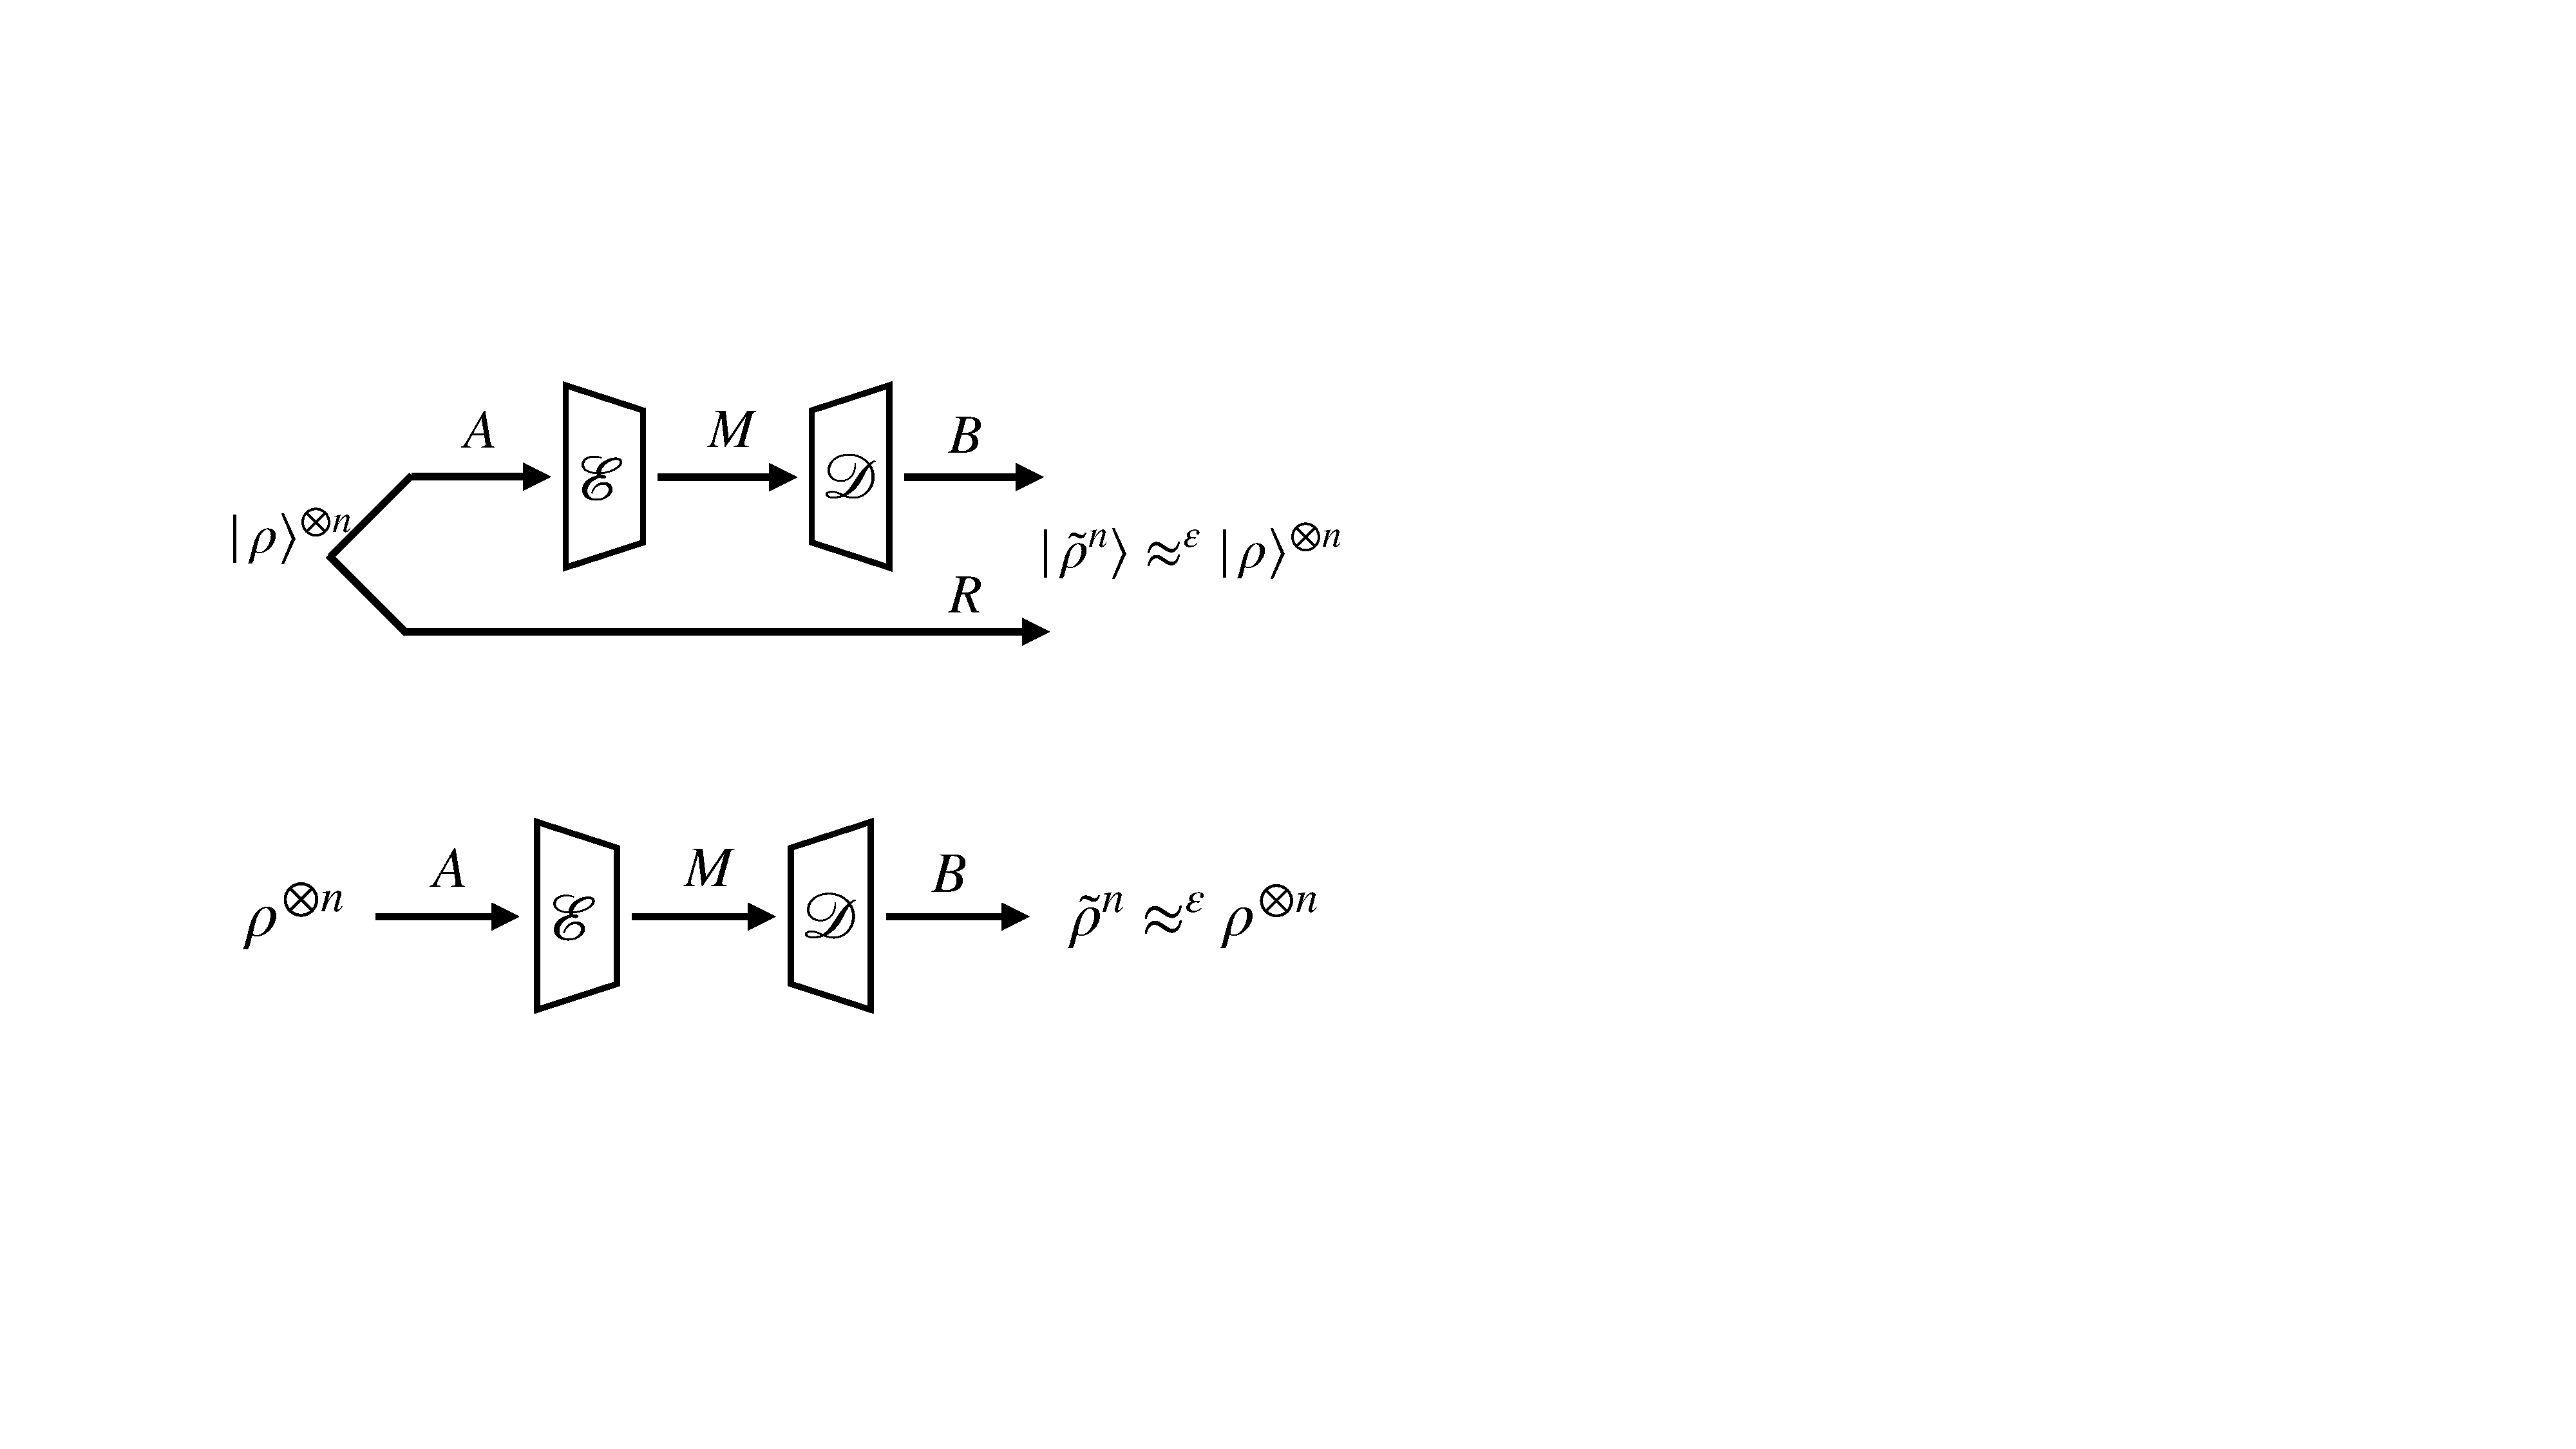
\includegraphics[width=1.0\linewidth]{compression.pdf}
    \caption{\label{fig:compression} \textbf{A variant of Schumacher compression.} The diagram above illustrates Schumacher compression, where the decoded state must preserve its purification. The diagram below illustrates our compression task that does not demand the purification to be preserved, and thus the memory $M$ only stores a quantum minimum description of the density operators $\rho^{\otimes n}$.}
\end{figure}

This compression task has previously been studied by one of us in~\cite{yang2016optimal,yang2018compression}~\footnote{Also, a classical version is studied in~\cite{hayashi2017minimum}.}, \YY{Should we cite a complete list on this sort of compression (I can add other references), or should we leave it to the long paper?}\JW{Either way.} with the focus on the leading order asymptotic compression rate of order $O(\log n)$. We are the first to identify the second order for qudits. While the second order rate is practically less important, it turns out to be theoretically more interesting, as we saw that the leading order term is universal, whereas the second order term is state-dependent and unveils itself as the free entropy.
 

What about the general case of compressing states with an unknown spectrum? This is also studied in~\cite{yang2016optimal,yang2018compression} at the leading order, and the answer is $|M| = \frac{d^2-1}{2}\log n$. Is it also relate to the physical free entropy?  The second order, however, would be less interesting because without knowing anything about the state, the QMDL would just be a universal state-independent number. Nonetheless, the leading order behavior does match the physical free entropy. If we focus only on the leading term in~\ref{eq:free_phys}, we have $\chi_\mathrm{phy}(\rho;\eps)\simeq d^2\delta(\rho)\log\eps^{-1}$. For $\rho$ with an unknown spectrum, we have $d^2\delta(\rho) = d^2-1$ because it has $d^2-1$ degrees of freedom. Therefore, the result of~\cite{yang2016optimal,yang2018compression} reads $|M| =\frac12\chi_\mathrm{phy}(\rho;n^{-1})$ up to a constant.

%Conclusion

%Kolmogorov Complexity
\emph{Discussion}---The QMDL of $\rho^{\otimes n}$ can also be understood as the quantum Kolmogorov complexity of the family of states $\{(U\rho_0 U^\dagger)^{\otimes n}\}_{U\in \text{U}(d)}$~\footnote{The exact definition of quantum Kolmogorov complexity does not matter here. cf.~\cite{mueller2007} for more details.}. It describes the descriptive complexity of  $\rho^{\otimes n}$. A similar result, concerning only the pure state case, is mentioned in two proposals of quantum Kolmogorov complexity (cf. Theorem 7 in~\cite{Berthiaume_2001} and Theorem 15 in~\cite{G_cs_2001}). The classical analog of $\rho^{\otimes n}$ is a repetitive string, which has Kolmogorov complexity of $\log n + O(1)$. This is because we only need $O(1)$ amount of bits to describe each chuck of the string and use another $\log n$ bits to describe how long the string is. Our result is structurally similar: it has the universal $\log n$ scaling and all the features of the state is stored in the $O(1)$ piece. However, we note that, because of the no-cloning theorem, there are some discrepancies between the classical and quantum results. The quantum Kolmogorov complexity only converges to the $O(\log n)+O(1)$ form asymptotically, and it has a $\frac12\log n$ contribution per degree of freedom.



% Free entropy vs vN entropy
We would like to close by highlighting two important distinctions of free entropy from quantum entropy. 

Firstly, von Neumann entropy only makes sense when the notion of density operator makes sense, which might not be available in infinite dimensions, whereas free entropy is defined on the more general object of non-commutative distribution, i.e., collection of correlators. When it comes to multivariate entropies, their distinction becomes clearer. The latter is more versatile because correlators are always defined, but density operators are not always available when dealing with non-commuting systems of observables. 

This versatility allows one to talk about free entropy of not only density operators describing states, but also of unitary operators describing unitaries or Hermitian operators describing observables. Therefore, the operational meaning of QMDL we found for density operators can in principle be generalized to other contexts. 

We conjecture that free entropy describes the quantum minimum description length of any operator in quantum mechanics. The relevant information-theoretic task is therefore the task of \emph{programming}, which asks for the minimum size of quantum memory needed to store a universal program for any instance drawn from a family of operators. The problem of universal programming has been studied for unitaries and measurements up to the leading order~\cite{Kubicki_2019,yang2020optimal,DAriano_2005,PrezGarca_2006}. We believe that the free entropy shall show up in the second order rate of the program size—capturing the state-dependent operational fluctuations—just as we find it for the density operators.

Secondly, as for why it is called free entropy, ``free'' refers to \emph{freeness}, or free independence. This is an alternative notion of independence for quantum (non-commutative) random variables. Freeness does not have a classical analog, and it is genuinely tied with non-commutativity. The freeness between two operators can be roughly understood as saying that the two operators have no algebraic relations with each other. In other words, knowing one operator does not help us describe the other. 

Crucially, free entropy is extensive (additive) under free independence modeled by the free product, whereas von Neumann entropy is extensive under tensor independence as modeled by the tensor product~\cite{speicher1996universal}. \YY{Can we move this earlier as a motivation for this study?}\JW{Idk what's the best way to do it, because we don't have more to say about freeness and additivity and we only study single-variate entropy.} This is the most distinctive feature of free entropy. We only found the operational meaning of the free entropy of one variable. We expect that the multivariate free entropy is the quantum minimum description length of multiple operators given we know all their relations. Free entropy is thus subadditive because at worst we can describe them individually, and equality is achieved when there are no relations between free operators that we can exploit.

In physics, freeness pertains to the independence between observables separated across time under chaotic dynamics, whereas tensor independence pertains to the independence between observables separated across space. Hence, we expect the utility of free entropy and related free entropic quantities in characterizing quantum information in quantum dynamics. A recent work by one of us showcases how \emph{free mutual information} can be useful in probing quantum chaos and serving as mutual information across time~\cite{vardhan2025}. The free mutual information can also characterize how scrambling unitary channels are, despite that they all have maximal quantum channel capacities.

Overall, the free entropy theory provides a new perspective to study quantum information in a way that is complementary to quantum entropies. Given the strong parallel between free entropy theory and the classical and quantum theory of entropies, we envision that a new kind of information theory will be revealed.

\begin{acknowledgments}
We would like to thank Geoff Penington, Shreya Vardhan and Edward Witten for discussions about free entropy.
\end{acknowledgments}


\appendix

\section{Physical free entropy}\label{sec:regularize}
\YY{If we are submitting to PRL, we can have 2 pages of End Matter (two-column), which makes all content appear in the same document and is better than SI imo. Can we compress the appendix a bit?}\JW{Sounds good!}
In this appendix, we provide the derivation of the physical free entropy formula and briefly introduce the concept of free entropy dimension.

To rigorously define the physical free entropy, we replace the continuous Lebesgue measure with the metric entropy (or Kolmogorov $\eps$-entropy) of the space of viable microstates. Let $\Omega_\eps$ be the subset of the $d^2$-dimensional real vector space of Hermitian matrices $M_d^{\mathrm{s.a.}}$ that satisfies our spectral condition:
\begin{equation}
    \Omega_\eps \equiv \left\{ X_d \in M_d^{\mathrm{s.a.}} \, \big\vert \, \| \lambda(X_d) - p \|_2 \le \eps \right\}
\end{equation}
where $\lambda_i$ and $p_i$ denote the ascending eigenvalues of $X_d$ and $\rho$, respectively. 

We equip $M_d^{\mathrm{s.a.}}$ with the Euclidean metric induced by the Hilbert-Schmidt inner product, $\langle A, B \rangle = \Tr(A B)$. The number of $\eps$-distinguishable microstates is given by the $\eps$-covering number of $\Omega_\eps$, denoted $\mathcal{N}(\Omega_\eps, \eps)$, which is the minimum number of balls of radius $\eps$ required to cover $\Omega_\eps$. We define the physical free entropy directly via this covering number:
\begin{equation}
    \chi_{\mathrm{phy}}(\rho; \eps) \equiv \log \mathcal{N}(\Omega_\eps, \eps)
\end{equation}

To evaluate this, we utilize standard volumetric bounds from high-dimensional geometry. If we cover $\Omega_\eps$ with $\mathcal{N}(\Omega_\eps, \eps)$ balls of radius $\eps$, the sum of their volumes bounds the total volume of $\Omega_\eps$. Let $B_\eps^{d^2}$ denote the $d^2$-dimensional Euclidean ball of radius $\eps$, whose Lebesgue volume scales as $\mathrm{Vol}(B_\eps^{d^2}) = C_{d^2} \eps^{d^2}$, where $C_{d^2}$ is the volume of the unit ball. For small $\eps$, the covering number satisfies the tight asymptotic relation:
\begin{equation}
    \mathcal{N}(\Omega_\eps, \eps) \simeq \frac{\mathrm{Vol}(\Omega_\eps)}{\mathrm{Vol}(B_\eps^{d^2})}\ .
\end{equation}

We evaluate $\mathrm{Vol}(\Omega_\eps)$ using eigenvalue-eigenvector coordinates. Because our integration domain restricts the eigenvalues to be ordered ascendingly ($\lambda_1 \le \dots \le \lambda_d$), the map to the unordered diagonal matrix is one-to-one, so we use the ordered Lebesgue measure on $M_d^\mathrm{s.a.}$:
\begin{equation}
    \dd X = c_d\prod_{1\le i<j\le d}(\lambda_i-\lambda_j)^2\dd\lambda_1\cdots\dd\lambda_d \,\dd\nu(U)
\end{equation}
where the integration constant is $c_d =\pi^{d(d-1)/2}/\prod_{k=1}^{d-1} k!$. 

Because we bounded the eigenvalue $L_2$ deviation by $\eps$, the ordered eigenvalue integration domain $D_\eps$ is identical to a $d$-dimensional Euclidean ball $B_\eps^d(p)$, which has the volume $\mathrm{Vol}(D_\eps) = \pi^{d/2}\eps^d/\Gamma(d/2 + 1) $. 

For sufficiently small $\eps$, the volume of the spectral neighborhood is heavily dominated by the value of the Vandermonde determinant evaluated at the fixed spectrum $p$:
\begin{multline}
    \mathrm{Vol}(\Omega_\eps) \simeq c_d \, \mathrm{Vol}(D_\eps) \Delta(p) = \\\frac{\pi^{d(d-1)/2}}{\prod_{k=1}^{d-1} k!} \frac{\pi^{d/2}}{\Gamma(d/2 + 1)} \eps^d \prod_{1\le i<j\le d}(p_i-p_j)^2\ .
\end{multline}

Notice that the total power of $\pi$ in the numerator is $\pi^{d(d-1)/2 + d/2} = \pi^{d^2/2}$. We now divide this by the reference Euclidean cell volume, which is the volume of the $d^2$-dimensional ball $B_\eps^{d^2}$:
\begin{equation}
    \mathrm{Vol}(B_\eps^{d^2}) = \frac{\pi^{d^2/2}}{\Gamma(d^2/2 + 1)} \eps^{d^2}\ .
\end{equation}

When taking the ratio to find the covering number, the $\pi^{d^2/2}$ factors perfectly cancel:
\begin{multline}
    \mathcal{N}(\Omega_\eps, \eps) \simeq \frac{\mathrm{Vol}(\Omega_\eps)}{\mathrm{Vol}(B_\eps^{d^2})} =\\ \frac{\Gamma(d^2/2 + 1)}{\Gamma(d/2 + 1) \prod_{k=1}^{d-1} k!} \eps^{-(d^2-d)} \prod_{1\le i<j\le d}(p_i-p_j)^2\ .
\end{multline}


Taking the logarithm yields the physical free entropy, exposing the exact Euclidean artifacts alongside the topological representation constant:
\begin{multline}\label{eq:free_phys1_app}
    \chi_{\mathrm{phy}}(\rho; \eps) = (d^2-d)\log \eps^{-1} + 2\sum_{1\le i<j\le d} \log|p_i-p_j|\\ - \sum_{k=1}^{d-1} \log k! + \log \left( \frac{\Gamma(d^2/2 + 1)}{\Gamma(d/2 + 1)} \right) + O(\eps)\ .
\end{multline}

If the spectrum is degenerate, the volume is different. Let the distinct eigenvalues of $\rho$ be $p_1<\cdots<p_m$ with multiplicities $g_1,\ldots,g_m$ and $\sum_a g_a=d$. Let the smallest gap between the eigenvalues be $g$ and let $\eps<g/2$. 

For $\lambda\in D_\eps$, we label and group the eigenvalues as consecutive blocks indexed by $i=(a,r)$:
\begin{equation}
    \lambda_{a,1}\le\cdots\le\lambda_{a,g_a},\quad a=1,\ldots,m\ ,
\end{equation}
and we set
\begin{equation}
    \lambda_{a,r} = p_a+x_{a,r}\ .
\end{equation}
This split is possible because $\eps<g/2$ so the blocks are cleanly centered around $p_a$'s and do not overlap.

Then $\Delta(\lambda)$ breaks into the inter-block term and the intra-block term:
\begin{equation}
    \Delta(\lambda) = \prod_{a<b}\prod_{r=1}^{g_a}\prod_{s=1}^{g_b}(\lambda_{b,s}-\lambda_{a,r})^2\cdot
    \prod_{a=1}^m\prod_{1\le r<s\le g_a}(\lambda_{a,s}-\lambda_{a,r})^2\ .
\end{equation}

Because we bounded the spectral distance by $\eps$, we roughly have $|x_{a,r}|\le \eps$ for $\lambda\in D_\eps$\ .

The inter-block term becomes
\begin{multline}
    \prod_{a<b}\prod_{r=1}^{g_a}\prod_{s=1}^{g_b}(p_b-p_a +(x_{b,s}-x_{a,r}))^2
     \\=\prod_{a<b}(p_b-p_a)^{2g_ag_b} + O(\eps)\ ,
\end{multline}
and the intra-block term becomes
\begin{equation}
     \prod_{a=1}^m\prod_{1\le r<s\le g_a}(x_{a,s}-x_{a,r})^2\ .
\end{equation}
Let $x=\eps y$ and $y=O(1)$, the intra-block term becomes
\begin{equation}
    \prod_{a=1}^m\eps^{g_a(g_a-1)}\prod_{1\le r<s\le g_a}(y_{a,s}-y_{a,r})^2\equiv \eps^{\sum_a g_a(g_a-1)}W(y)\ ,
\end{equation}
where we pulled out the $\eps$-dependent term.

The volume integral follows similarly, absorbing the integral over $W(y)$ and the related topological artifacts into the geometric constant:
\begin{multline}
   \mathrm{Vol}(\Omega_\eps) \simeq \prod_{a<b}(p_b-p_a)^{2g_ag_b} \int_{D_\eps} \eps^{\sum_ag_a(g_a-1)} W(y) \eps^d\dd y \\
   =\eps^{\sum_ag_a^2}\prod_{a<b}(p_b-p_a)^{2g_ag_b} \int W(y)\dd y + O(\eps)\ .
\end{multline}

The physical free entropy formula reads,
\begin{multline}\label{eq:degenerate_free_ent}
    \chi_\mathrm{phys}(\rho;\eps) = \left(d^2 - \sum_a g_a^2\right)\log \eps^{-1} \\+ 2\sum_{a<b}g_a g_b\log |p_a-p_b| + \mathrm{const} + O(\eps)
\end{multline}
The second term is equal to $\chi_\mathrm{reg}(\rho)$ in~\eqref{eq:reg_free_ent}.

This formula~\eqref{eq:degenerate_free_ent} reduces to~\eqref{eq:free_phys1_app} when all $g_a=1$. The coefficient $d^2 - \sum_a g_a^2$ is the number of degrees of freedom for a density operator with spectral degeneracies~$g_a$. 

\begin{comment}
    
\end{comment}
There is a complementary heuristic to derive formula~\eqref{eq:degenerate_free_ent}. We can take the divergent formula~\eqref{eq:free_ent_formula} and regularize it by smearing the density matrix with some random noise. In free probability, this is usually done by adding a freely independent \emph{semicircular} $s$ to $\rho$~\footnote{A freely independent \emph{semicircular} $s$ is approximately an independent random GUE matrix.}. A semicircular $s$ is defined to have the moments of the semicircular distribution, and is the non-commutative analog of a Gaussian.

The spectral density of $\rho+\eps s$ can be calculated using the free additive convolution. Its support has as many disconnected domains as the number of distinct eigenvalues, and each domain has a width of order $\eps$~\cite{biane1997free}. The resulting free entropy admits the following expansion at small $\eps$
\begin{align}
    \label{eq:smeared_free_ent}
    \chi(\rho+\eps s)
    =\frac{\sum_ig_i^2}{d^2}\log\eps+ \chi_\mathrm{reg}(\rho) + \mathrm{const} + O(\eps)\ .
\end{align}


Now we recall that the physical free entropy~\eqref{eq:free_phys_def} is defined using the metric entropy $\mathcal{N}(\Omega_\eps, \eps)$ that factors out a universal $d^2\log\eps^{-1}$ term. This regularized free entropy above identifies a divergent piece in $\chi(\rho)$: $\frac{\sum_ig_i^2}{d^2}\log\eps$.  We can now absorb it into the $d^2\log\eps^{-1}$ term. We thus obtain the physical free entropy formula~\eqref{eq:degenerate_free_ent}
\begin{equation}
    \chi_\mathrm{phy}(\rho;\eps)=\left(d^2-\sum_ig_i^2\right)\log\eps^{-1} + \chi_\mathrm{reg}(\rho) + \mathrm{const} + O(\eps).
\end{equation}
Hence, the physical free entropy $\chi_\mathrm{phy}(\rho;\eps)$ can be treated as a regularized quantity. The bare divergence in $\chi(\rho)$ can be absorbed into the universal divergent term.

To see the most general formula~\eqref{eq:free_phys} holds, we need to introduce the concept of free entropy dimension. When the bare free entropy diverges, the submanifold has dimension $d^2-\sum_ig_i^2$, fewer than $d^2$. In free entropy theory, this dimension is formally known as the \emph{free entropy dimension}, which generalizes the Minkowski dimension (or entropy dimension) to the non-commutative setting. 

For an operator $a\in(\A,\tau)$, the free entropy dimension is defined as 
\begin{equation}\label{eq:fed}
    \delta(a)\equiv 1+\lim_{\eps\to 0}\frac{\chi(a+\eps s)}{-\log\eps}
\end{equation}
where $a$ and the semicircular $s$ are free. The semicircular smearing helps to remove any logarithmic divergences from the free entropy, and the limit extracts the degree of the divergences and subtracts them from $1$. We have $0\leq\delta(a)\leq 1$ and $\delta(a)=1$ iff $\chi(a)>-\infty$. 

We can substitute~\eqref{eq:smeared_free_ent} into~\eqref{eq:fed}, and we see that the free entropy dimension is exactly the factor controlling the leading $\log\eps^{-1}$ term in the definition of physical free entropy. We hence obtain~\eqref{eq:free_phys}:
\begin{equation}\label{eq:free_phys'}
    \chi_\mathrm{phy}(\rho;\eps)=d^2\delta(\rho)\log\eps^{-1} + \chi_\mathrm{reg}(\rho) + \mathrm{const} + O(\eps)\ ,
\end{equation}
and we can confirm that by explicitly calculating the free entropy dimension for various cases. For a single variable, the free entropy dimension has a formula that subtracts from $1$ the contributions from the atoms~\cite{voiculescu2002free}
\begin{equation}
    \delta(a)=1-\sum_{t\in\mathbb{R}} \mu_a(\{t\})^2
\end{equation}
where $\mu_a$ is the spectral measure of $a$. Using this formula, we can work out some simple examples: For a rank-$k$ $d$-dimensional projector $P$,
\begin{equation}\label{eq:proj_fed_ex}
    \delta(P)=2\frac{k}d\left(1-\frac{k}d\right)\ .
\end{equation}
For a $d$-dimensional Hermitian operator $\rho$ that has spectral degeneracies $g_i$, where $i$ labels distinct eigenvalues, we have
\begin{equation}\label{eq:fed_ex}
    \delta(\rho)=1 - \sum_i\frac{g_i^2}{d^2}\ .
\end{equation}
which gives exactly~\eqref{eq:free_phys1} when substituted in~\eqref{eq:free_phys'}.

\section{Free entropy of density operators with a degenerate spectrum}\label{sec:degeneracy}
For a density operator with spectral degeneracy, the free entropy is given in~\eqref{eq:degenerate_free_ent}. Our result for QMDL in~\cite{paper2} is a bit more general than that stated in the main text. We could also allow $\rho$ to be rank-deficient, as long as the non-zero eigenvalues are non-degenerate. Let the rank of $\rho$ be $r$ and thus null space dimension of $\rho$ be $d-r$, so the degeneracies are the zero eigenvalue be $g_0 = d-r$ and $g_{i\ge 1}= 1$. We have
\begin{multline}
    \chi_\mathrm{phys}(\rho;\eps) = r\left(2d-r-1\right)\log \eps^{-1}  + 2\sum_{1\le i<j}\log |p_i-p_j| \\ + 2(d-r)\sum_{i\ge 1}\log p_i + \mathrm{const} \ ,
\end{multline}
and it characterizes the QMDL of any rank-deficient $\rho$,
\begin{equation}
    |M| = \frac{1}{2}\chi_\mathrm{phy}(\rho,n^{-1}) + \mathrm{const} + o(1)\ .
\end{equation}

We leave the details to the companion paper~\cite{paper2}, but it is useful to discuss the case of a pure state. The density operator of a pure state is a rank-1 projector $\ketbra{\psi}{\psi}$, so $r=d-1$ and $p_0=0, p_1=1$. We have
\begin{equation}
    \chi_\mathrm{phys}(\ketbra{\psi}{\psi};\eps) = (2d-2)\log \eps^{-1} + \mathrm{const}
\end{equation}
which agrees with the free entropy dimension calculated in~\eqref{eq:free_phys'}$(k=1)$, and the logarithmic potential term vanishes on $\log 1$.

The QMDL of $\ketbra{\psi}{\psi}^{\otimes n}$ is thus $(d-1)\log n$ at large $n$, because we only need to compress to the symmetric subspace, which has dimension $O(n^{d-1})$.

We expect that with a more careful analysis for $\rho$ with a degenerate spectrum, the QMDL of any density operator $\rho^{\otimes n}$ can be shown to be the free entropy~\eqref{eq:degenerate_free_ent}.


\bibliographystyle{apsrev4-2}
\bibliography{free}

\end{document}